\documentclass[paper=a4]{article}
\usepackage{tikz}
%\usetikzlibrary{decorations}
\usetikzlibrary{decorations.pathmorphing,calc}
\begin{document}


\begin{figure}[H]
\begin{centering}
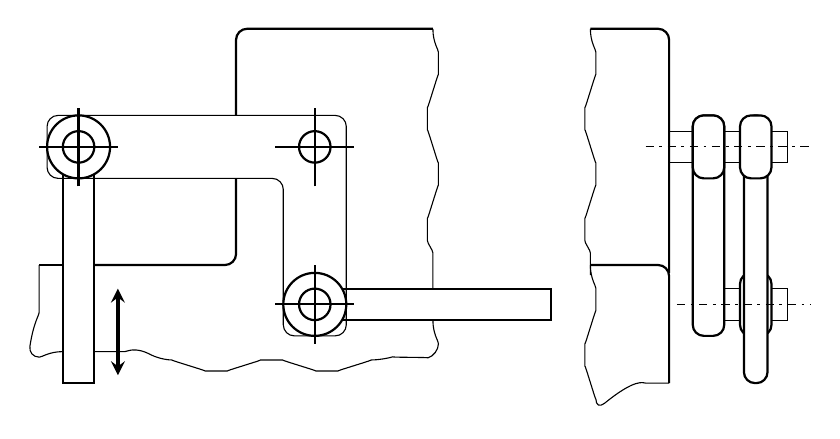
\begin{tikzpicture}

	\newcommand{\drawcircle}[3]{\draw[#3] (#1,#2) circle(0.2);
		\draw[#3] ($(#1,#2)+(-0.5,0)$)--($(#1,#2)+(0.5,0)$);
		\draw[#3] ($(#1,#2)+(0,-0.5)$)--($(#1,#2)+(0,0.5)$);};

\drawcircle{-3}{0}{ thick};
\drawcircle{0}{0}{ thick};
\drawcircle{0}{-2}{ thick};

%Gestaenge
\draw[rounded corners] (-3.4,0.4)--(0.4,0.4)--(0.4,-2.4)--(-0.4,-2.4)--(-0.4,-0.4)--(-3.4,-0.4)--cycle;
\draw[thick] (-3,0) circle(0.4);
\draw[thick] (-3.2,-0.35)--(-3.2,-3)--(-2.8,-3)--(-2.8,-0.35);

\draw[thick] (0,-2) circle(0.4);
\draw[thick] (0.35,-2.2)--(3,-2.2)--(3,-1.8)--(0.35,-1.8);

\draw[rounded corners,thick](-2.8,-1.5)--(-1,-1.5)--(-1,-0.4) ;

\draw[rounded corners,thick](-1,0.4)--(-1,1.5)--(1.5,1.5);
\draw[rounded corners,thick](-3.5,-1.5)--(-3.2,-1.5);

\draw[rounded corners, decorate, decoration ={ snake , segment length =40, amplitude =2}] (1.5,1.5)--(1.5,-1.8);

\draw[rounded corners, decorate, decoration ={ snake , segment length =40, amplitude =2}] (1.5,-2.2)--(1.5,-2.6)--(-2.8,-2.6);


\draw[rounded corners, decorate, decoration ={ snake , segment length =40, amplitude =2}] (-3.2,-2.6)--(-3.5,-2.6)--(-3.5,-1.5);

\draw[stealth-stealth , very thick] (-2.5,-1.8)--(-2.5,-2.9);

%%%%%%%%%%%%%%%%%%%%%%%%%%%%%%%%%%%%%%%%%%%%%
%%%%%%%%%%%%%%Seitenansicht%%%%%%%%%%%%%%%%%%
%%%%%%%%%%%%%%%%%%%%%%%%%%%%%%%%%%%%%%%%%%%%%

\draw[thick, rounded corners] (3.5,1.5)--(4.5,1.5)--(4.5,-1.6);
\draw[rounded corners,thick] (3.5,-1.5)--(4.5,-1.5)--(4.5,-3); 
\draw[rounded corners, decorate, decoration ={ snake , segment length =40, amplitude =2}] (3.5,1.5)--(3.5,-1.5);

\draw[rounded corners, decorate, decoration ={ snake , segment length =40, amplitude =2}](3.5,-1.5)--(3.5,-3)--(4.5,-3);

\draw[] (4.5,0.2) rectangle (6,-0.2);
\draw[] (4.8,-2.2) rectangle (6,-1.8);


\draw[rounded corners, thick, fill=white] (4.8,-2.4) rectangle (5.2,.4);
\draw[rounded corners, thick, fill=white] (4.8,-.4) rectangle (5.2,.4);

\draw[rounded corners, thick, fill=white] (5.4,-2.4) rectangle (5.8,-1.6);
\draw[rounded corners, thick, fill=white] (5.45,.4) rectangle (5.75,-3);
\draw[rounded corners, thick, fill=white] (5.4,-.4) rectangle (5.8,.4);

\draw[dash pattern= on 3pt off 2pt on 1pt off 2pt] (4.2,0)--(6.3,0);
\draw[dash pattern= on 3pt off 2pt on 1pt off 2pt] (4.6,-2)--(6.3,-2);


\end{tikzpicture}
\par\end{centering}
\caption{Hebelgest\"ange mit Quetschgefahr}
\end{figure}



\end{document}